%!TEX root = ../../thesis.tex

The SM is a gauge quantum field theory describing the kinematics and interactions of 
sub-atomic particles 
\cite{Aitchison,Peskin,Glashow:1961,Weinberg:1967,Salam:1968,'tHooft:1972}. 
The dynamics of such a theory are determined 
by the symmetries respected by its Lagrangian. The SM is invariant under local 
transformations of the \SMgroup gauge group, resulting in the strong, weak and 
electromagnetic forces of nature. Additionally, invariance under global transformations of 
the Poincaré group ensures the theory is identical in all inertial frames of reference, as 
asserted by special relativity.

Each constituent gauge theory of the SM describes the dynamics of a force of nature, 
which is mediated by a number of gauge bosons and couples to a conserved current, in 
accordance with Noether's theorem \cite{Noether:1918}. Quantum chromodynamics (QCD) of 
\SUgroup{3} describes the strong interaction, is mediated by eight gluons, and couples to 
colour charge. Quantum electrodynamics (QED) of \Ugroup{1} describes the electromagnetic 
interaction, is mediated by the photon, and couples to electric charge. The weak 
interaction is mediated by the massive \PWpm and \PZ bosons and is best understood within 
the context of the electroweak (EW) theory, a unification of the electromagnetic and weak 
interactions. A theory of gravity is not included in the SM. Significantly, the gauge 
groups of the strong and weak interactions are non-abelian. Physically, this means that 
the gauge bosons are themselves charged and therefore experience self-interactions.

\begin{figure}[t]
	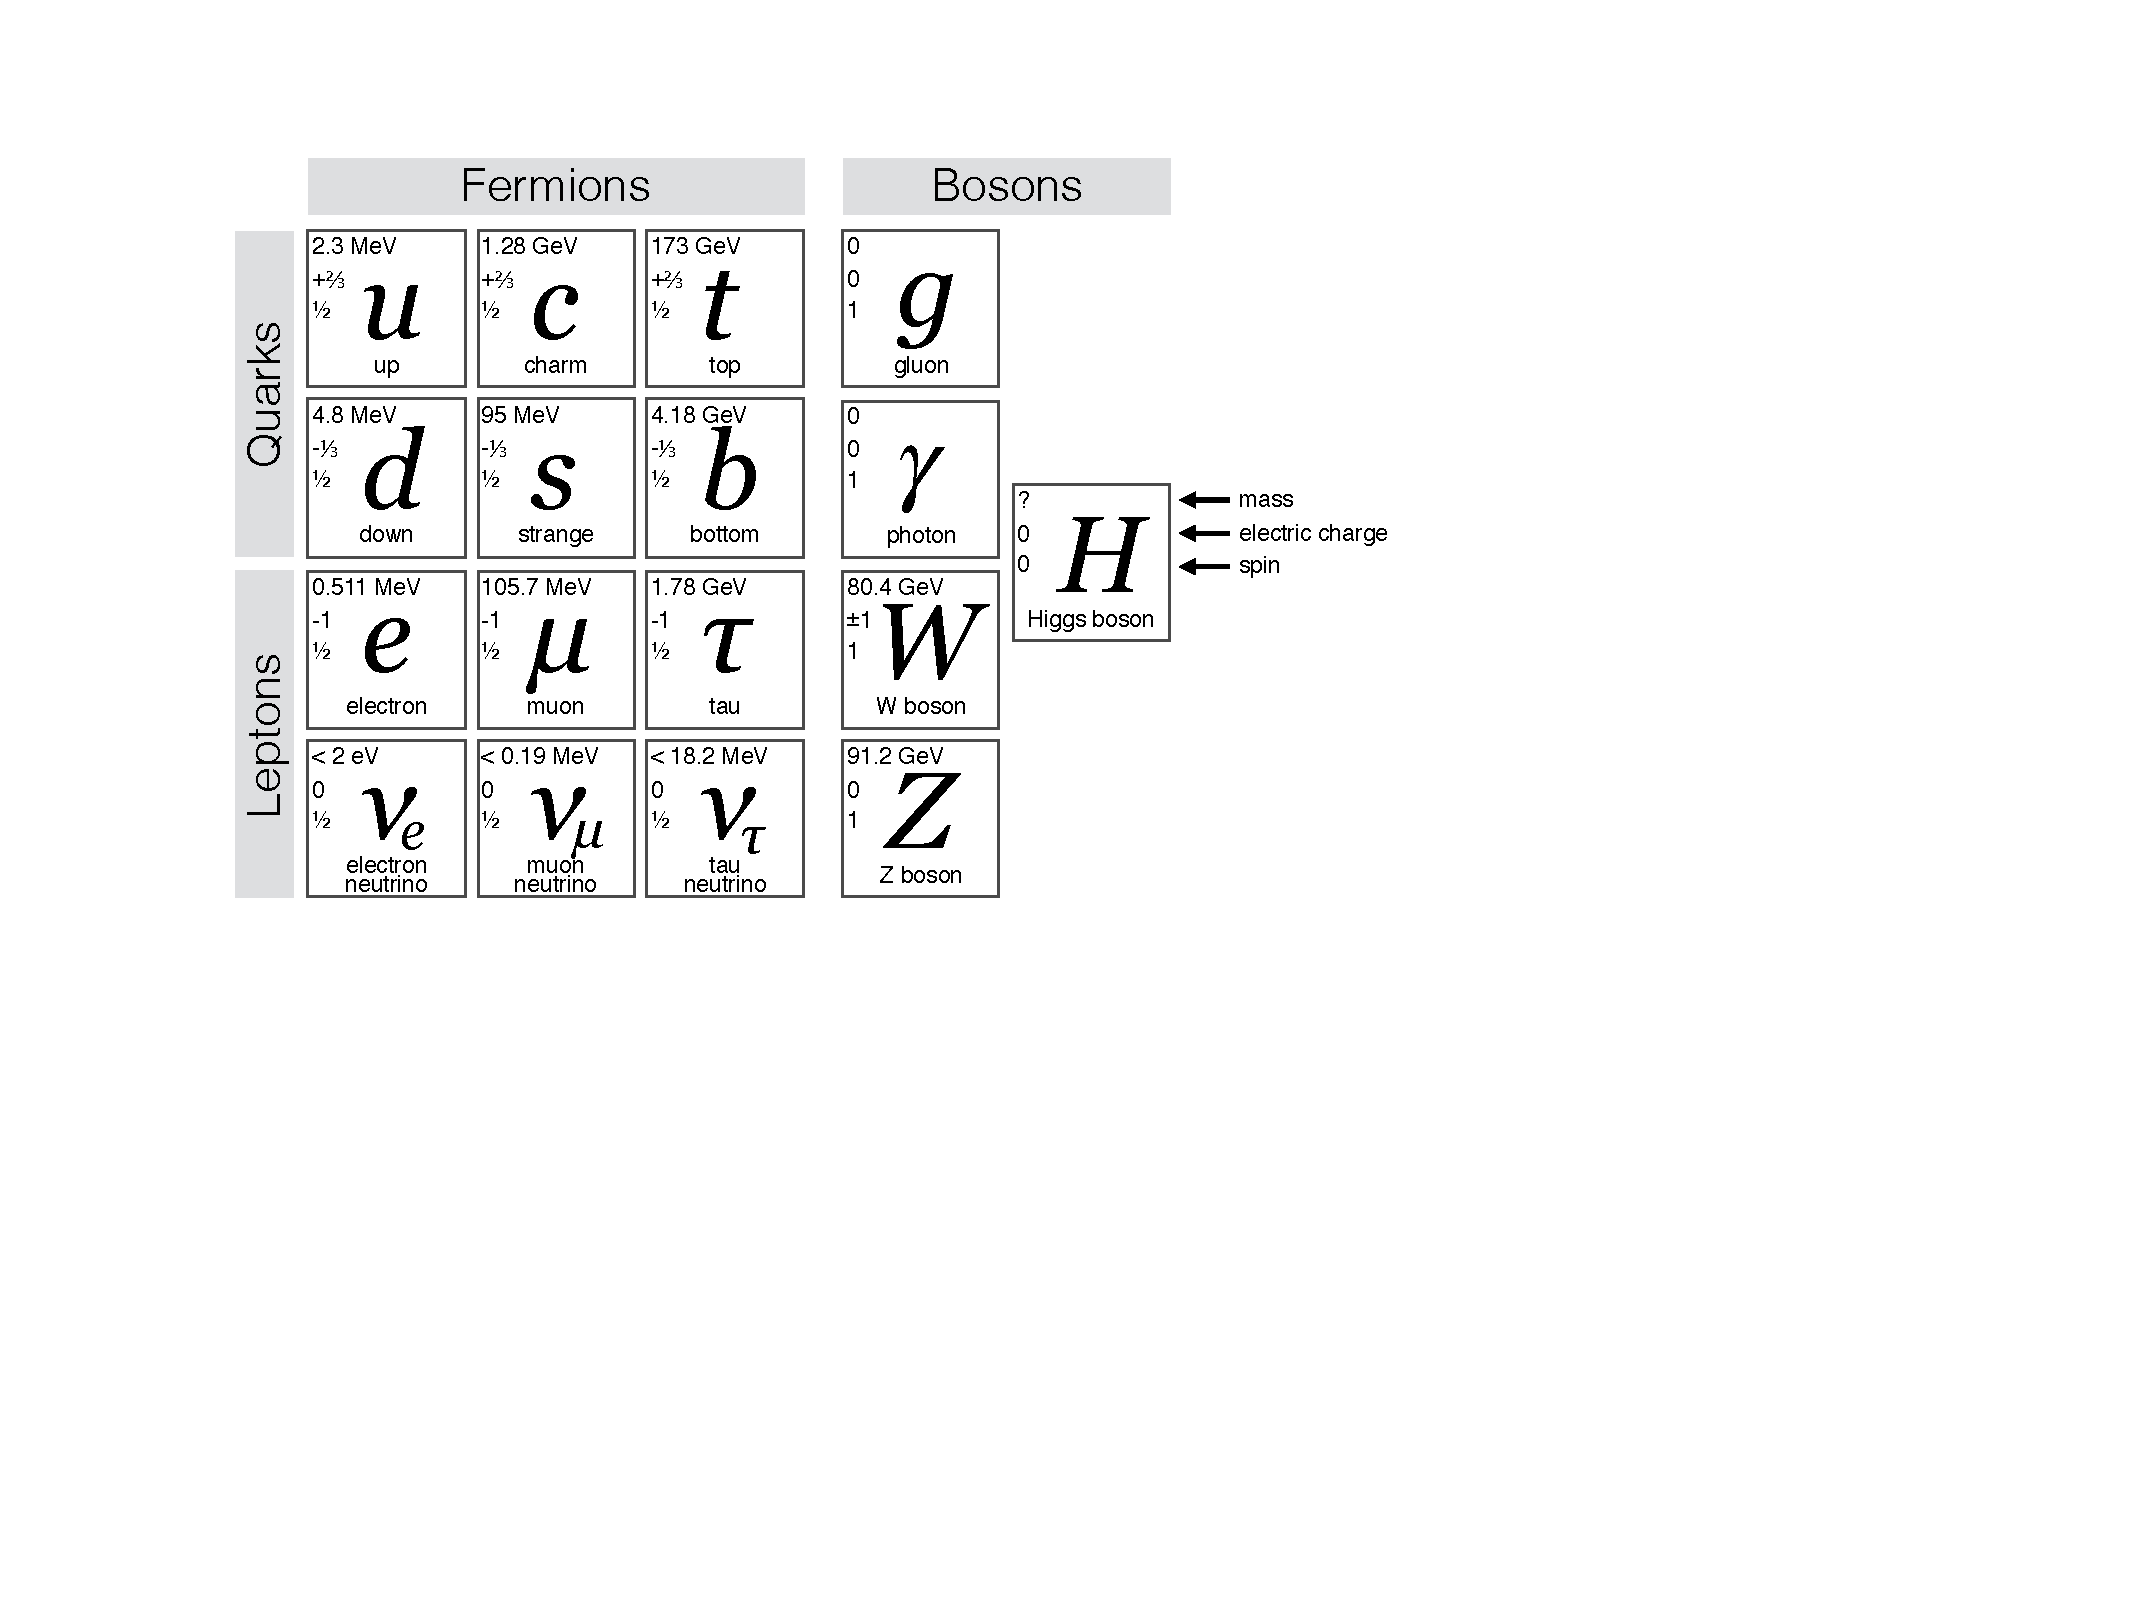
\includegraphics[width=\largefigwidth,clip=true,trim=3.9cm 11.8cm 12.6cm 2.6cm]{custom_images/sm_particles}
	\caption{The particle content of the SM, with masses from \cite{PDG:2012}. 
	Constraints upon the mass of the Higgs boson are described in 
	\Section~\ref{sec:prior_constraints}.}
	\label{fig:sm_particles}
\end{figure}

The elementary particles of the SM are summarised in \Figure~\ref{fig:sm_particles}.
They are categorised into bosons (integer spin) and fermions (half-integer spin).
In addition to the gauge bosons introduced above, the Higgs boson is a by-product
of electroweak symmetry breaking (described in \Section~\ref{sec:ewsb}) and couples to 
mass. The twelve flavours of fermions are categorised according to the interactions they 
experience, or equivalently the charges they possess: quarks (strong, electromagnetic, 
weak), charged leptons (electromagnetic, weak) and neutrinos (weak). The fermions are also 
arranged in three generations of increasing mass. Massive particles can decay into less 
massive particles, while obeying the conservation laws of the SM. Fermions have an 
associated antiparticle with identical mass but inverted internal quantum numbers.
Isolated quarks are not observed; they form colourless composite particles called hadrons.
